\documentclass[screen]{beamer}
\usepackage[T1]{fontenc}
\usepackage[utf8]{inputenc}
\usetheme{ntnubokmaal}
 
\title[Problemstilling MiA]{Problemstilling for Futhark, MiA 2011}
\subtitle{Steking av bacon i mikrobølgeovn}
\author[Futhark]{Å. Ervik, K. H. Skrede, T. S. Solberg, P. Vo, J. Johnsen}
\institute[NTNU]{Eksperter i Team, NTNU}
\setbeamertemplate{footline}[ntnu theme nologo]
\date{09.02.2011}

\newcommand{\gv}[1]{\ensuremath{\mbox{\boldmath$ #1 $}}}
\renewcommand{\div}[1]{\gv{\nabla} \cdot #1} % for divergence
\newcounter{saveenumi}
%\newcommand{\labelitemi}{$\bullet$}

\begin{document}
\ntnutitlepage

\begin{frame}
  \frametitle{Problemstilling}
  \begin{center}
  \begin{itemize}  
  \item[$\bullet$] Hvordan kan steking av bacon i en mikrobølgeovn modelleres matematisk? 
  \item[$\bullet$] Hvordan vil fett-, vann- og saltinnhold påvirke stekingen, og hvilken effekt er optimal? 
  \end{itemize}
  \end{center}
\end{frame}

\begin{frame}
  \frametitle{Motivasjon}
  \begin{center}
  \begin{figure}[!h]
    \begin{center}
      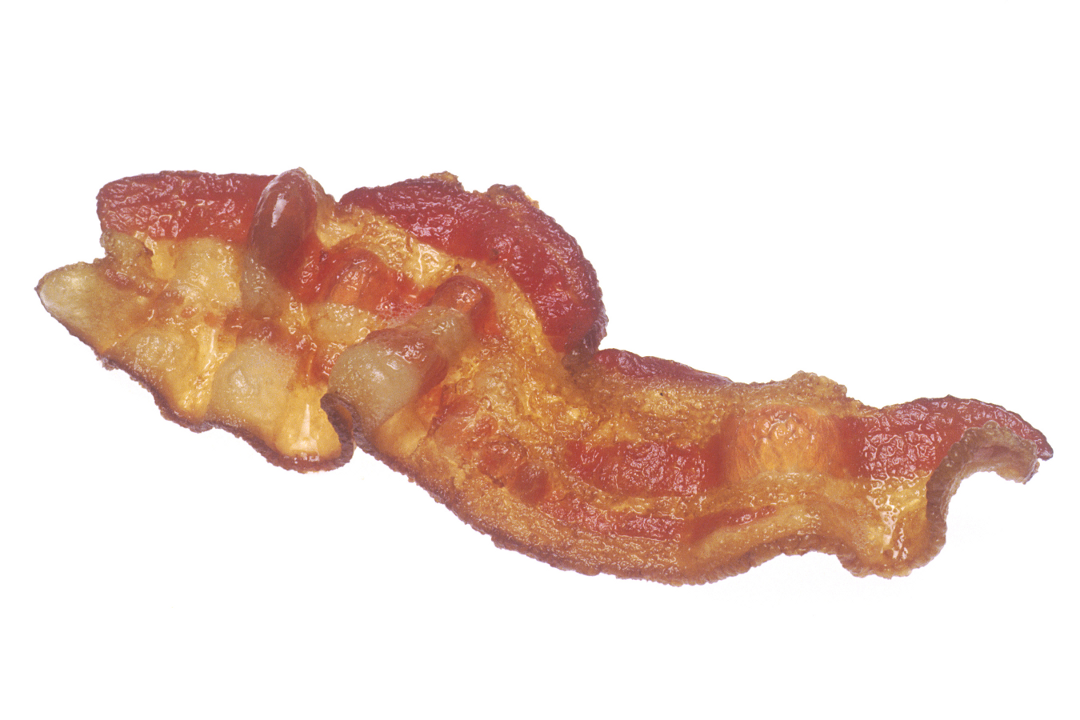
\includegraphics[width=0.6\textwidth]{bacon.png}
    \end{center}
    \caption{Mmmmm\ldots}
  \end{figure}
  \end{center}
\end{frame}


\begin{frame}
  \frametitle{Input og output}
  \textbf{Input:}
  \begin{itemize}
  \item[$\bullet$] vann-, fett- og saltinnhold
  \item[$\bullet$] geometri - tykkelse
  \item[$\bullet$] antall baconstriper
  \item[$\bullet$] effekt
  \item[$\bullet$] (ønsket sprøhet)
  \end{itemize}
  \textbf{Output:}
  \begin{itemize}
    \item[$\bullet$] steketid
  \end{itemize}
\end{frame}

\begin{frame}
  \frametitle{Modellen}
  \begin{enumerate}
  \item Varme
  \item Massetransport
  \item Nøyaktige grensebetingelser for mikrobølgeovn
    \setcounter{saveenumi}{\theenumi}
\end{enumerate}
    \hline
\begin{enumerate}
    \setcounter{enumi}{\thesaveenumi}
  \item Elektromagnetiske grensebetingelser
  \item App - redusert modell
  \end{enumerate}
\end{frame}

\begin{frame}
  \frametitle{Utgangspunkt}
  \begin{itemize}
    \item[$\bullet$] Massebevaring: $\rho_0 \frac{\partial u_i}{\partial\tau} =
      -\div{j_i} + I_i $ \vspace{10pt}
    \item[$\bullet$] Energibevaring: $c\rho_0\frac{\partial T}{\partial \tau} =
      -\div{q} + \displaystyle\sum\limits_{i} h_i I_i -
      \displaystyle\sum\limits_{i} j_i c_i {\gv\nabla} T$
    \item[$\bullet$] Varmelikning: $\frac{\partial u}{\partial \tau} = \alpha
      {\gv\nabla}^2 u$
    \item[$\bullet$] \vspace{10pt} Størrelser:
      \begin{itemize}
	\item $q = -\lambda {\gv \nabla } T$, $\lambda$ effektiv varmeledning
	\item $u_i$ masseinnholdet av damp (vann) i stoff $i$ (f.eks. kjøtt, fett)
	\item $j_i$ massestrømningstetthet for stoff $i$
	\item $I_i$ kilder og sluk pga. faseoverganger, $\displaystyle\sum\limits_{i} I_i = 0$
	\item $h_i$ varmen (termisk energi) i stoff $i$
	\item $c_i = \frac{\partial h_i}{\partial T}$ (varmekapasitet)
	\item $c = c_0 + \displaystyle\sum\limits_{i} c_i u_i$, $c_0$ varmekapasitet for tørt legeme
      \end{itemize}
  \end{itemize}
\end{frame}

\begin{frame}
  \frametitle{Løsningsmodell}
  \begin{itemize}
    \item[$\bullet$] Vi har tenkt å bruke Finite Difference Method (FDM) til å løse differensial-
lignignene presentert i forrige slides.

\item[$\bullet$] Planen er å bruke et vanlig grid i første omgang, for så og eventuelt forbedre
det, eksempelvis ved bruk av senterpunkter. For å sikre stabilitet har vi valgt
å bruke Crank-Nicolson:

\item[$\bullet$] 
\begin{equation*}
  \frac{u_i^{n+1}-u_i^n}{\Delta t} = \frac{1}{2(\Delta x)^2}((
  u_{i+1}^{n+1}-2u_i^{n+1}+u_{i-1}^{n+1}) \\ \hspace{110pt} + (u_{i+1}^{n} - 2u_i^n +
  u_{i-1}^{n}) ) 
\end{equation*}
  \end{itemize}
\end{frame}

\begin{frame}
  \frametitle{Løsningskriterier}
  \begin{center}
  \begin{itemize}  
    \item[$\bullet$] Hva får vår numeriske modell
      til å avslutte simuleringen?

\item[$\bullet$] Massedifferanse: Baconpakning gir fettinnholdet ved start,
  massetransportligninger gjør det mulig å finne kritisk massetap (målt gjennom forsøk).

\item[$\bullet$] Temperatur: Maillards reaksjoner sier at bruning starter ved
  154$^o$C. Kritisk temperatur.
  \end{itemize}
  \end{center}
\end{frame}

\begin{frame}
  \frametitle{Kalibrering}
  \begin{itemize}
	\item[$\bullet$] Måle effekt i mikrobølgeovnen ved å sette inn vannbad og måle hvor mye
	som fordamper i løpet av en gitt tid
        \item[$\bullet$] Sammenlikne med teoretisk effekt (f.eks. 750 W)
  \end{itemize}
\end{frame}

\begin{frame}
  \frametitle{Eksperimentell verifikasjon}
  \begin{itemize}
	\item[$\bullet$] Lese av innholdsfortegnelsen til baconet og egenskapene til mikrobølgeovnen
	og bruke disse som parametre
	\item[$\bullet$] Gjøre den matematiske berigningen av modellen med de gitte parametrene
	\item[$\bullet$] Stek bacon i mikrobølgeovnen med resultatet (tiden) gitt fra beregningen
	\item[$\bullet$] Dokumenter forventet resultat og faktisk resultat
	\item[$\bullet$] Gjenta N ganger
  \end{itemize}
\end{frame}

\end{document}

